\documentclass[10pt,a4paper,twoside,twocolumn]{article}
%% Lots of packages !
\usepackage{etex}

%% Francisation
\usepackage[english]{babel}
\usepackage[T1]{fontenc}
\usepackage[utf8]{inputenc}
%\usepackage{textcomp}

%% Réglages généraux
\usepackage[left=1.5cm,right=1.5cm,top=2cm,bottom=2cm]{geometry}
\usepackage{fancyhdr}
\usepackage{setspace}
\usepackage{lscape}
%\usepackage{multicol}
\usepackage{makeidx}
\usepackage[clearempty]{titlesec}
\usepackage{cite}

%% Packages pour le texte
\usepackage{pifont}
\usepackage{eurosym}
\usepackage{soul}
\usepackage[normalem]{ulem}
\usepackage{fancybox}
\usepackage{boxedminipage}
\usepackage{enumerate}
\usepackage{verbatim}
\usepackage{moreverb}
\usepackage{listings}
\usepackage[table]{xcolor}

%% Packages pour les tableaux
\usepackage{array}
\usepackage{multirow}
\usepackage{tabularx}
\usepackage{longtable}

%% Packages pour les dessins
\usepackage{graphicx}
\usepackage{wrapfig}
%\usepackage{picins}
\usepackage{picinpar}
\usepackage{epic}
\usepackage{eepic}
\usepackage{tikz}
\usepackage{afterpage}
\usepackage{rotating}
\usepackage{float}
\usepackage{caption}

%% Packages pour les maths
\usepackage{amsmath}
\usepackage{amssymb}
\usepackage{dsfont}
\usepackage{mathrsfs}
\usepackage{bussproofs}
\usepackage[thmmarks,amsmath]{ntheorem}

%% Création de nouvelles commandes
%\usepackage{calc}
\usepackage{ifthen}
\usepackage{xspace}



\usepackage{url}
\usepackage{hyperref}
\usepackage{todonotes}
\usepackage{subcaption}
\usepackage[french,ruled,vlined,linesnumbered,algosection,dotocloa]{algorithm2e}
\usepackage{MnSymbol}

\usepackage{chngcntr}

\usepackage{standalone}
\usepackage{import}

\usepackage[affil-it]{authblk}


\usepackage{lipsum}












\numberwithin{equation}{subsection}


\newcommand*{\rootPath}{../}
\standalonetrue

\begin{document}

\section{Pipeline description}
The main objective of the pipeline is to build an analyse a density field from a
sampling representing the  density field. In real application this sampling can
be data comming from the acquisition of a real experiment or the the result of a
simulation program such as the Hacc cosmology simultation code\todo{ref}.

\begin{figure}[!ht]
	\centering
	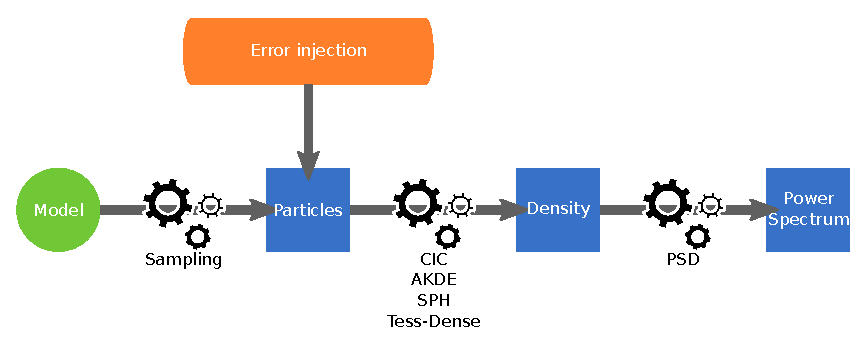
\includegraphics[width=0.4\textwidth]{\rootPath Figures/model-pipeline.eps}
	\caption{Full pipeline}
	\label{fig:pipeline}
\end{figure}

\subsection{Syntetic particles generation}

In order for us to have a good idea of the expected results, we will use
syntetic particles generated by the sampling of an analytical distribution with
caracteristics close to thoses expected from the real application values. That
way we have analytical values helping us compared all our results to a known
ground truth.

This analytical distribution is a density profil produced by a sum of
Navarro-Frenk-White functions\cite{navarro96}. This density profile is further
caracterized in \todo{ref - Self-Adaptive Density Estimation of Particle Data}.
$$\mathcal D(p) = \sum_{\{k_i, c_i\}} \frac{k_i}{\|p-c_i\|(\|p-c_i\|+1)^2}$$

We will also use values produced by real application in order to confirm the
results comming from the synthetic particles.

\subsection{Density estimation}

Density estimation aims at reconstructing the density function from a set of
samples. This is achieved by adding the contribution of all sample, each sample
representing a local density profile. The distribution of this local density
profile is caracteristed by a weighting function and by a domain, which
caracteristics have been extensivelly studied
\todo{ref - Self-Adaptive Density Estimation of Particle Data}.

However, more accurate methods also tends to be more computationnaly expensive
and not so qualitative methods tends to be prefered in cases where intermediate
quality results are satisfactory and computation cost needs to be limited.

We therefore will consider different methods representing differents compromise
between results quality and computation cost.

\subsection{Density analysis}

In order to compare different density fields produced by the density estimation
methods, we need a metric caracterising the representative elements of those
density fields. This metric should differentiate values according to the
relevant elements in regard to their futher analysis in real application.

For this step, the use a power spectrum analysis which makes visible variation
responses for different caracteristic length, hence detecting bias such as high
frequency noise or over smoothness. In order to compare distances between those
spectral responces we use the following integral based metric :
$$d(ps_1, ps_2) = \int_{\Delta f}\frac{\|ps_1(f)-ps_2(f)\|^2}{f}\, \mathrm df$$
By dividing by the frequency we ensured a constant contribution from all orders
of magnitudes. This notably helps discriminate variation at low frequencies and
therefore check total weight of the density field.

%=====================================================================
%=====================================================================
\ifstandalone
	\bibliographystyle{apalike}
	\bibliography{\rootPath Annexes/biblio}
\fi
%=====================================================================
%=====================================================================
\end{document}
